\section{Experimental validation}
\label{sec:exps}

We experimented our models on several real world networks, directed and undirected. Theirs statistics and properties are summarized in table \ref{table:corpus} and detailed descriptions are available in the online Koblenz network collection\footnote{http://konect.uni-koblenz.de/networks/}. For both astro-ph and hep-ph datasets, we used the cleaned version available in the  graph-tool framework.
%The aim of these experiments is to illustrate the advantage of the online inference and to evaluate the performances of the models.

\begin{table}[h]
\bgroup
\def\arraystretch{1} % 1 is the default, change whatever you need
	
\caption{Datasets networks used to train the models. Type A is for co-authorship, type C is for communication, type H is for hyperlinks, type L is for lexical network and I for interaction network.}

\resizebox{\textwidth}{!}{
\begin{tabular}{lrrrrcrrrr}
%\Xhline{2\arrayrulewidth}
\toprule
 Datasets     &   Nodes &   Edges &   Density & Directed  &    Diameter &   \multicolumn{3}{c}{Weights}  	& type     \\
 \cmidrule(l){7-9}  &   &   	  &   $\times 10^{-3}$		  & 		  &  		   	&  mean & std  & max             \\
%\hline
\midrule
astro-ph      & 16,706  & 121,251   & 0.87  & False & 14 & 1.8  & 3.3  & 306  & A  \\
%cond-mat     & 16,726  & 47,594    & 0.000 & False & 18 & 3.1  & 7.2  & 544  & A  \\
hep-th        & 8,361   & 15,751    & 0.45  & False & 1  & 5.2  & 16   & 1226 & A  \\
%netscience   & 1,589   & 2,742     & 0.002 & False & 2  & 2.2  & 1.9  & 33   & A  \\
moreno\_names & 1,773   & 9,131     & 5.81  & False & 8  & 1.8  & 3.0  & 100  & L  \\
manufacturing & 167     & 5,783     & 208   & True  & 3  & 14.3 & 44.9 & 1458 & C  \\
fb\_uc        & 1,899   & 20,296    & 5.63  & True  & 4  & 2.8  & 4.7  & 98   & C  \\
digg\_reply   & 30,398  & 85,247    & 0.09  & True  & 11 & 2.0  & 0.2  & 26   & C  \\
slashdot      & 51,083  & 130,370   & 0.05  & True  & 11 & 2.1  & 0.3  & 18   & C  \\
enron         & 87,273  & 320,154   & 0.04  & True  & 15 & 3.4  & 12.4 & 3904 & C  \\
wiki-link     & 100,312 & 887,426   & 0.09  & True  & 14 & 1.7  & 3.0  & 185  & H  \\
prosper-loans & 89,269  & 3,330,225 & 0.42  & True  & 2  & 2.0  & 0.2  & 16   & I  \\
%\Xhline{2\arrayrulewidth}
\bottomrule
\end{tabular}
}


\egroup
\label{table:corpus}
\end{table}

\subsection{Experimental setup}
As standard in social network analysis, the evaluation of the models is based on the missing link prediction task using the AUC-ROC score. For weighted models, we consider the probability that an edge exists between two unobserved nodes $(i,j)$ belonging to the test set, namely:
\[
p(y_{ij} \geq 1 | \Thetah, \Phih) = 1 - \sum_{kk'} \thetah_{ik} \thetah_{jk'} e^{\phih_{kk'}}
\]

For all the datasets, we built a test set by extracting randomly 20 percent of the edges of the network and about the same amount of non-links. The remaining data constitutes the "full" training set. Then, in order to assess how the models behave when few training data is available, we sub-sampled this full training set in order to obtain smaller sub-training sets (subgraphs) containing different proportions of the edges (i.e 1\%, 5\%, 10\%, 20\%, 30\%, 50\%, and 100\%). Note that we ensure that all the sub-training sets are inclusive. We repeated this sampling 10 times with different seeds to cross validate our results. The average values (and standard deviations) computed on the ten sub-training sets are reported, for each proportion, as final results.

% stopping citerion
For deciding when to stop the inference process, 10\% of the training set used serves as a validation set on which the log-likelihood is computed after each minibatch iteration. When the increase of the log-likelihood, averaged over the last 20 measures, is less than 0.001, the inference is stopped. The log-likelihood of a given set of observations $\D_{set}$  is given by:
\begin{equation*}
\log p(\D_{set}) = \sum_{i,j \in \D_{set}} \log p(y_{ij} | \phih_{kk'}) p(k|\thetah_i) p(k'|\thetah_j)
%\log p(\D_{test}) = \sum_{i,j \in \D_{test}} \log p(y_{ij} | \phih_{kk'}) p(k|\thetah_i) p(k'|\thetah_j)
\end{equation*}

For all our models, the gradient step parameters  $\tau$ and $\kappa$ were fixed respectively to  $1024$ and $0.5$, the burn-in period $T_{burnin}$ to $150$; for stratified sampling, $M$ was set to $50$, the size of $s_0^{i,m}, \, 1 \le m \le M$ being equal to the number of nodes to which $i$ is not connected to divided by $M$. For MMSB, the hyperparameters $\lambda_0$ and $\lambda_1$ were set to $0.1$. For WMMSB, the shape and scale parameters $r$ et $p$ were fixed to $1$ and for WMMSB, the beta-gamma hyperparameters were fixed to  $c_0=10$, $r_0=1$, $c=100$ and $\epsilon=10^{-6}$. The number of latent classes $K$ was fixed to $10$ for all models and the latent-class hyperparameters $\alpha_k$ to $\frac{1}{K}$. Our implementation is available online\footnote{https://github.com/***/*** (anonymized)}. In addition, we consider here two standard link prediction models, the stochastic block model, referred to as SBM, and its weighted extension, referred to as WSBM. For these two models, the microcanonical stochastic block model implementation of \cite{peixoto2018nonparametric} has been used since it integrates an efficient MCMC inference method for the stochastic block model family.  The number of classes was also set to $K=10$.

Variational inference, used here for MMSB models, and MCMC, used for SBM models, lead to different performance, the latter usually yielding better models than the former \cite{asuncion2009smoothing}. Indeed, despite the fact that the MMSB models considered here rely on more realistic assumptions regarding the distribution of nodes over latent classes, the approximations made on the likelihood for scalable inference purposes penalize MMSB models when it comes to prediction accuracy. This said, the strong averaging step of the stochastic gradient descent allows for faster convergence so that, as the models are more realistic, they may yield better performance when the amount of training data is limited. This is indeed what we observe in practice.

%\textcolor{white}{ % trick to make it invisible, only in the footpage.
%\footnote{\url{http://konect.uni-koblenz.de/networks/ca-AstroPh}. We used the cleaned version available in the  graph-tool framework.}
%\footnote{\url{hhttp://konect.uni-koblenz.de/networks/ca-cit-HepTh}. We used the cleaned version available in the  graph-tool framework.}
%\footnote{\url{hhttp://konect.uni-koblenz.de/networks/moreno_names}}
%\footnote{\url{hhttp://konect.uni-koblenz.de/networks/radoslaw_email}}
%\footnote{\url{hhttp://konect.uni-koblenz.de/networks/opsahl-ucsocial}}
%\footnote{\url{hhttp://konect.uni-koblenz.de/networks/munmun_digg_reply}}
%\footnote{\url{hhttp://konect.uni-koblenz.de/networks/slashdot-threads}}
%\footnote{\url{hhttp://konect.uni-koblenz.de/networks/enron}}
%\footnote{\url{hhttp://konect.uni-koblenz.de/networks/link-dynamic-simplewiki}}
%\footnote{\url{hhttp://konect.uni-koblenz.de/networks/prosper-loans}}
%}

\begin{figure}[h]
\centering
	
\begin{subfigure}
     \centering
         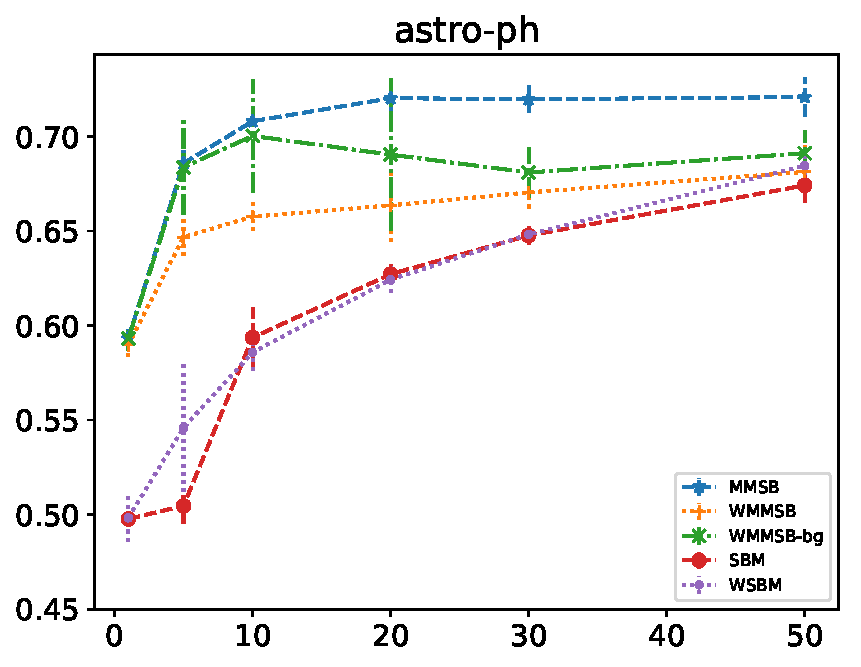
\includegraphics[width=0.32\textwidth]{fig/astro-ph__entropy@_roc_evo2}
\end{subfigure}
\begin{subfigure}
         \centering
      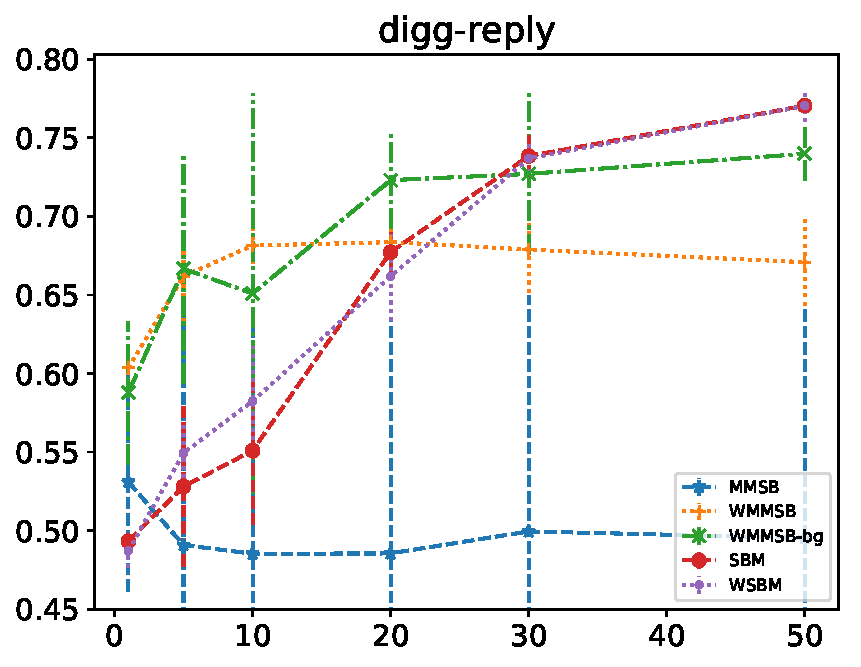
\includegraphics[width=0.32\textwidth]{fig/digg-reply__entropy@_roc_evo2}               
\end{subfigure}                                                                          
\begin{subfigure}                                                                        
         \centering                                                                      
      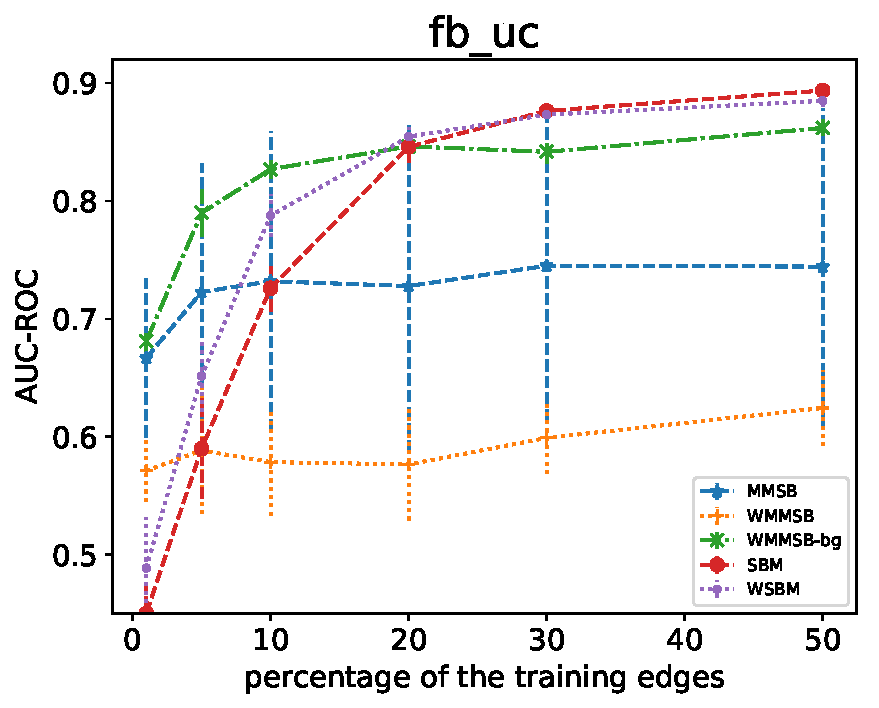
\includegraphics[width=0.32\textwidth]{fig/fb_uc__entropy@_roc_evo2}
\end{subfigure}                                                                          
\begin{subfigure}                                                                        
         \centering                                                                      
      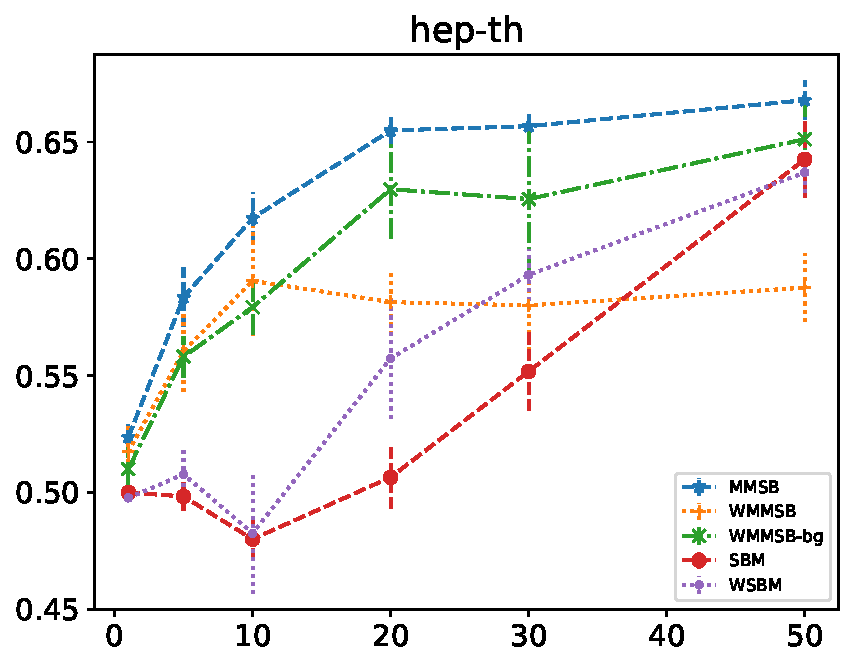
\includegraphics[width=0.32\textwidth]{fig/hep-th__entropy@_roc_evo2}
\end{subfigure}                                                                          
\begin{subfigure}
         \centering
      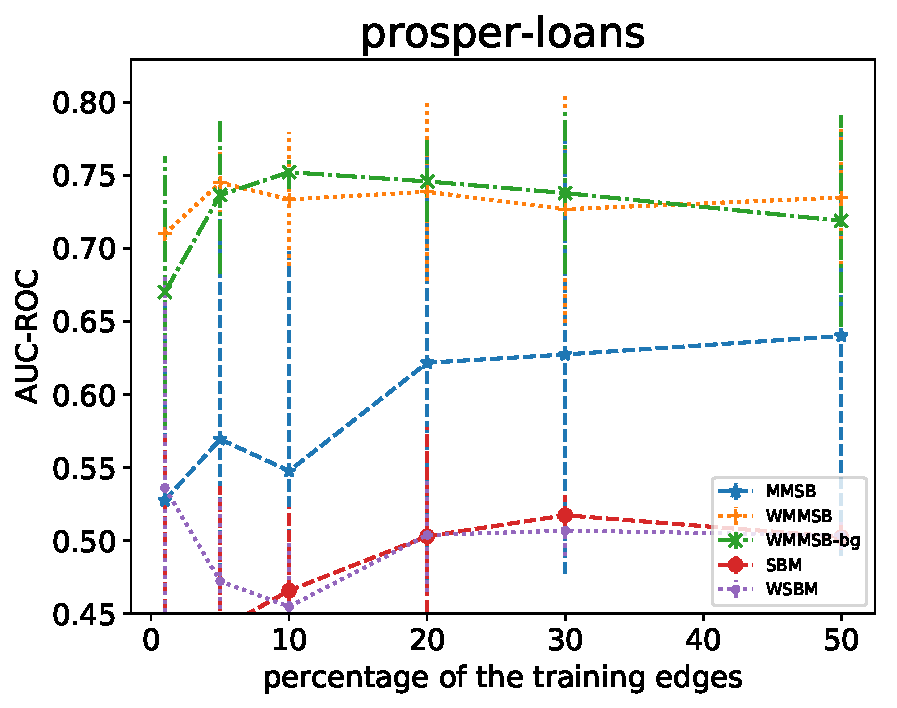
\includegraphics[width=0.32\textwidth]{fig/prosper-loans__entropy@_roc_evo2}
\end{subfigure}                                                             
\begin{subfigure}                                                           
         \centering                                                         
      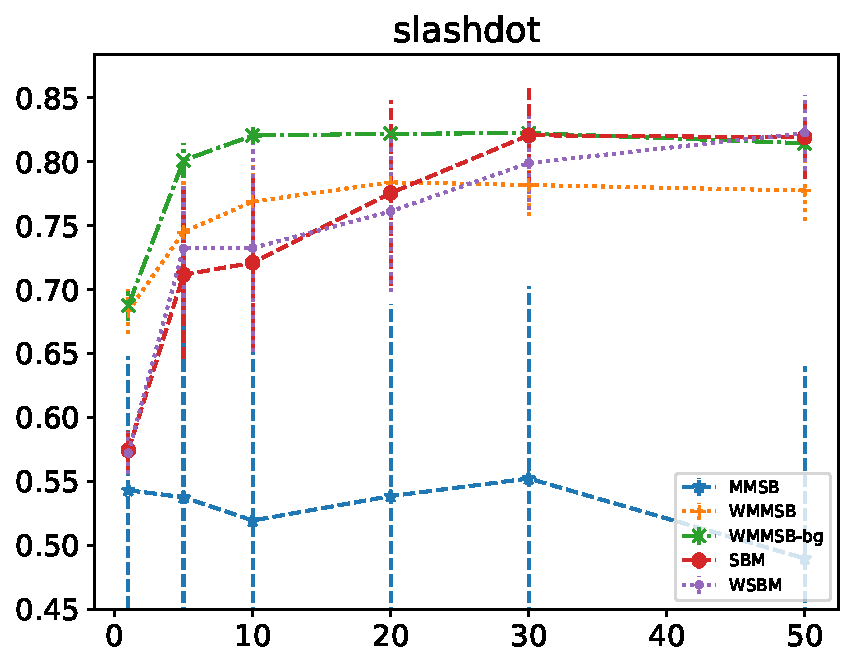
\includegraphics[width=0.32\textwidth]{fig/slashdot__entropy@_roc_evo2}
\end{subfigure}                                                             
\caption{Performance comparaison of models in terms of AUC-ROC score in function of the proportion of the observed edges used to train the models from 1 to 100 percent of the training set. Results are averaged on ten independant trials. Except for astro-ph and proper-loans where SBM and WSBM are not competitive, the curves cross each other at a specific proportion of training data under which MMSB, WMMSB and WMMSB-bg perfom better. }


   \label{fig:roc}
\end{figure}

\subsection{Results}
Figure \ref{fig:roc} gives the AUC/ROC scores for the different models when using 1\%, 5\%, 10\%, 20\%, 30\% and 50\% of the training data, for 6 networks (the complete results, over all training set size and networks are given in the supplementary material). As one can note, MMSB models outperform the other models when the amount of training data is limited. Among these models, WMMSB-bg is the best performing one, which highlights the importance of the Beta and Gamma priors used. The poor performance of MMSB on some networks can be explained by the fact that the convergence of the model is very sensitive to the sampling choices done during the online inference, as illustrated by the high variance in the results. When the amount of training data is sufficient (which depends on the network considered), SBM models tend to be better. As discussed before, we attribute this to the MCMC method used in SBM models. Surprisingly, and contrary to what is happening for MMSB models, WSBM does not really outperform SBM; this model does not seem to be able to make a good use of the edge covariates. 

Table~\ref{table:roc}, which displays the results of MMSB, WMMSB-bg, SBM and WSBM for all networks when using 10\% and 100\% of the training data, confirms these elements. As one can note, using all training data, SBM outperforms WSBM on 5 datasets. Interestingly, there is an important degradation for SBM models when only 10\% of the training set is used. MMSB models are more stable in this aspect, showing that the stochastic variational inference used in MMSB models allows one to learn a correct model with few data.

Finally, it is worth mentioning that on the dataset prosper-loans, the only network classified as "Interaction" in the Konnect repository, most models fail to learn the topology. In particular, MMSB barely exceeds a random classifier. Only the weighted MMSB models, WMMSB and WMMSB-bg, succeed in predicting new edges, with a performance above 0.75 when using only 10\% of the training data.
 
%MMSB is competitive on some datasets (astro-ph, hep-th, moreno\_names) while it fails on the others. Interestingly, one can see than on the datasets where it fails (digg-reply, prosper-loans, slashdot and wiki-link), the variance is very large. This behavior could be exploited to indicate if the model is suited for capturinfg the structure of a given network. Furthermore, those datasets have a low density compared to astro-ph, hep-th and moreno\_names. Thus, this poor performance can be explained by the fact that the convergence of the model is very sensitive to the sampling choices done during the online inference. Indeed, sparse networks are known to exhibit a degree distribution following a power law, which implies that some nodes do not have the same importance but the sampling does not integrate this property. In this regard, WMMSB and WMMSB-bg models are less sensitive for those networks and are still competitive. This result confirm  that taking into account the edge covariates makes the weighted models less sensitive to the minibatches sampling in sparse networks. Finally, it worth to mention that on the dataset prosper-loans, which is the only network classified as "Interaction" network in the Konnect repository, the baselines failed to learn the topology of the networks and MMSB barely exceeds a random classifier; only WMMSB-bg succeeds with the best performance above 0.75.

% Table Roc comments
\begin{table}
\centering
	
\caption{AUC-ROC performance comparaison of the models. Each model has 2 columns corresponding to two subsamples of the full training set. The subsamble contains either 10 or 100 percent of the edges in the trainin set, and there are inclusive. The AUC value is performed on the testing set build from the initial dataset by extracting 20 percent of the edges and about the the same amount of non-edge. 
For each dataset we randomly build a unique training and testing set shared by all the model. The scores are averaged on 10 independents trials (for each trials we build a unique traning and testing set.) and scaled by a factor $10^{3}$ in the table. We bold the best results w.r.t the training set of 10 percent and we underline the best results w.r.t to the training set of 80 percent. The results show that the MMSB and WMMSB-bg with our inferenc scheme outperform SBM and WSBM when the number of observation is low. Furthermore WMMSB-bg outperforms MMSB on most of the datasets.}

%\resizebox{12cm}{!}{
\resizebox{\textwidth}{!}{

\begin{tabular}{lllll|llll}
\toprule
&   \multicolumn{2}{c}{MMSB} &   \multicolumn{2}{c}{WMMSB-bg} &   \multicolumn{2}{c}{SBM} & \multicolumn{2}{c}{WSBM}   \\
\cmidrule(l){2-3} \cmidrule(l){4-5} \cmidrule(l){6-7}\cmidrule(l){8-9}  & 10 & 100 & 10 & 100 & 10 &  100 & 10 & 100   \\
%\hline
\midrule                              
astro-ph        &  \textbf{708} $\pm$ 3    & \underline{716} $\pm$ 11          & 700 $\pm$ 30            &  710 $\pm$ 18   &   594 $\pm$ 16   &  701 $\pm$ 6               &   588 $\pm$ 12           & 705 $\pm$ 5  \\
hep-th          &  \textbf{617} $\pm$ 11   & 675 $\pm$ 8           & 579 $\pm$ 12            &  676 $\pm$ 8    &   480 $\pm$ 9    &  \underline{779} $\pm$ 1               &   497 $\pm$ 29            & 716 $\pm$ 9  \\
moreno\_names   &  680 $\pm$ 72            & 738 $\pm$ 33          & \textbf{707} $\pm$ 29   &  739 $\pm$ 7    &   571 $\pm$ 29   &  \underline{862} $\pm$ 7               &   588 $\pm$ 25            & 862 $\pm$ 10 \\
fb\_uc          &  732 $\pm$ 127           & 784 $\pm$ 14          & \textbf{827} $\pm$ 8    &  850 $\pm$ 20   &   726 $\pm$ 20   &  \underline{902} $\pm$ 2               &   787 $\pm$ 15            & 896 $\pm$ 2  \\
digg\_reply     &  485 $\pm$ 178           & 482 $\pm$ 204         & \textbf{651} $\pm$ 127  &  744 $\pm$ 15   &   551 $\pm$ 47   &  728 $\pm$ 26              &   584 $\pm$ 34            & 714 $\pm$ 17 \\
slashdot        &  519 $\pm$ 193           & 634 $\pm$ 181         & \textbf{820} $\pm$ 6    &  791 $\pm$ 11   &   721 $\pm$ 66   &  830 $\pm$ 16              &   699 $\pm$ 79            & \underline{833} $\pm$ 13 \\
enron           &  459 $\pm$ 289           & 529 $\pm$ 256         & \textbf{875} $\pm$ 14   &  835 $\pm$ 8    &   870 $\pm$ 80   &  799 $\pm$ 20              &   866 $\pm$ 45            & \underline{842} $\pm$ 51 \\
wiki-link       &  491 $\pm$ 242           & 432 $\pm$ 185         & 739 $\pm$ 73            &  785 $\pm$ 8    &   848 $\pm$ 4    &  \underline{925} $\pm$ 2               &   \textbf{853} $\pm$ 4    & 914 $\pm$ 4  \\
prosper-loans   &  548 $\pm$ 284           & 434 $\pm$ 274         & \textbf{752} $\pm$ 11   &  \underline{727} $\pm$ 30   &   466 $\pm$ 57   &  500 $\pm$ 4               &   455 $\pm$ 44  	       & 505 $\pm$ 5  \\

\bottomrule
\end{tabular}


}


          
          
          





% 5 20 100

%&   \multicolumn{3}{c}{MMSB} &   \multicolumn{3}{c}{WMMSB-bg} &   \multicolumn{3}{c}{SBM} & \multicolumn{3}{c}{WSBM}     \\
%\cmidrule(l){2-4} \cmidrule(l){5-7} \cmidrule(l){8-10}\cmidrule(l){11-13}  & 5 & 20 & 100 & 5 & 20 & 100 & 5 & 20 & 100 & 5 & 20 & 100   \\

%astro-ph        &  686 $\pm$ 7    & 720 $\pm$ 8    & 716 $\pm$ 11   & 684 $\pm$ 25 & 690 $\pm$ 40  &  710 $\pm$ 18   &    505 $\pm$ 9  &  627 $\pm$ 5   &  701 $\pm$ 6   &  538 $\pm$ 31  &    626 $\pm$ 9   & 705 $\pm$ 5  \\
%hep-th          &  583 $\pm$ 13   & 655 $\pm$ 6    & 675 $\pm$ 8    & 558 $\pm$ 9  & 630 $\pm$ 21  &  676 $\pm$ 8    &   498 $\pm$ 6   &  506 $\pm$ 13  &  779 $\pm$ 1   &  513 $\pm$ 24   &    545 $\pm$ 29  & 716 $\pm$ 9  \\
%moreno\_names   &  674 $\pm$ 43   & 740 $\pm$ 18   & 738 $\pm$ 33   & 664 $\pm$ 39 & 697 $\pm$ 33  &  739 $\pm$ 7    &   478 $\pm$ 59  &  698 $\pm$ 25  &  862 $\pm$ 7   &  457 $\pm$ 38   &    709 $\pm$ 9   & 862 $\pm$ 10 \\
%fb\_uc          &  723 $\pm$ 109  & 728 $\pm$ 140  & 784 $\pm$ 14   & 790 $\pm$ 20 & 846 $\pm$ 11  &  850 $\pm$ 20   &   590 $\pm$ 43  &  846 $\pm$ 13  &  902 $\pm$ 2   &  679 $\pm$ 27   &    855 $\pm$ 7   & 896 $\pm$ 2  \\
%digg\_reply     &  491 $\pm$ 150  & 486 $\pm$ 195  & 482 $\pm$ 204  & 667 $\pm$ 73 & 723 $\pm$ 31  &  744 $\pm$ 15   &   528 $\pm$ 51  &  677 $\pm$ 13  &  728 $\pm$ 26  &  554 $\pm$ 22   &    659 $\pm$ 26  & 714 $\pm$ 17 \\
%slashdot        &  537 $\pm$ 177  & 538 $\pm$ 186  & 634 $\pm$ 181  & 801 $\pm$ 13 & 822 $\pm$ 6   &  791 $\pm$ 11   &   712 $\pm$ 66  &  775 $\pm$ 72  &  830 $\pm$ 16  &  731 $\pm$ 64   &    733 $\pm$ 28  & 833 $\pm$ 13 \\
%enron           &  555 $\pm$ 300  & 576 $\pm$ 301  & 529 $\pm$ 256  & 862 $\pm$ 15 & 876 $\pm$ 9   &  835 $\pm$ 8    &   900 $\pm$ 3   &  898 $\pm$ 39  &  799 $\pm$ 20  &  887 $\pm$ 48   &    916 $\pm$ 29  & 842 $\pm$ 51 \\
%wiki-link       &  389 $\pm$ 192  & 505 $\pm$ 230  & 432 $\pm$ 185  & 749 $\pm$ 43 & 725 $\pm$ 87  &  785 $\pm$ 8    &   517 $\pm$ 59  &  870 $\pm$ 4   &  925 $\pm$ 2   &  592 $\pm$ 159  &    871 $\pm$ 2   & 914 $\pm$ 4  \\
%prosper-loans   &  569 $\pm$ 300  & 622 $\pm$ 233  & 434 $\pm$ 274  & 736 $\pm$ 54 & 746 $\pm$ 28  &  727 $\pm$ 30   &   439 $\pm$ 97  &  503 $\pm$ 74  &  500 $\pm$ 4   &  472 $\pm$ 59   &    504 $\pm$ 39  & 505 $\pm$ 5  \\

                     
                     
                     
                     
                     
                     
                     
                     
                     
               
               
                                                                                                                                        
                     
                                                                                                                                           
                     
                     
                                                                                                                                           
                     
                     
                     
                                                                                                                     









\label{table:roc}
\end{table}

%
% Convergence commments
%
\subsection {Convergence analysis} %We studied in a deeper way the convergence of WMMSB and WMMSB-bg models on the different datasets. 
Figure \ref{fig:conv_entropy} shows the evolution of the log-likelihood for the MMSB-based models on a validation set composed of 20\% of links and non-links for each network. We used three different sets for the hyperparameters shape $r$ and scale $p$ of WMMSB. Regardless of the values of these hyperparameters, one can observe that the augmented model WMMSB-bg is less prone to overfitting, usually converges to a better solution and only needs a small proportion of the total number $N^2$ of edges to do so.

\begin{figure}[h]
\centering
	

\begin{subfigure}
     \centering
         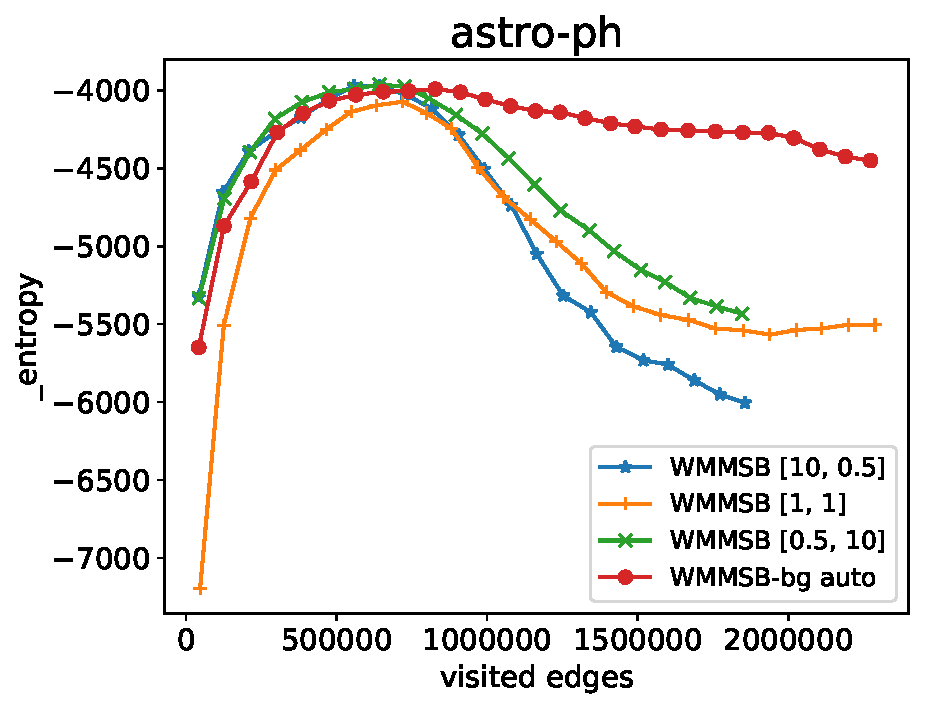
\includegraphics[width=0.32\textwidth]{fig/astro-ph_fig__entropy}
\end{subfigure}
\begin{subfigure}
         \centering
      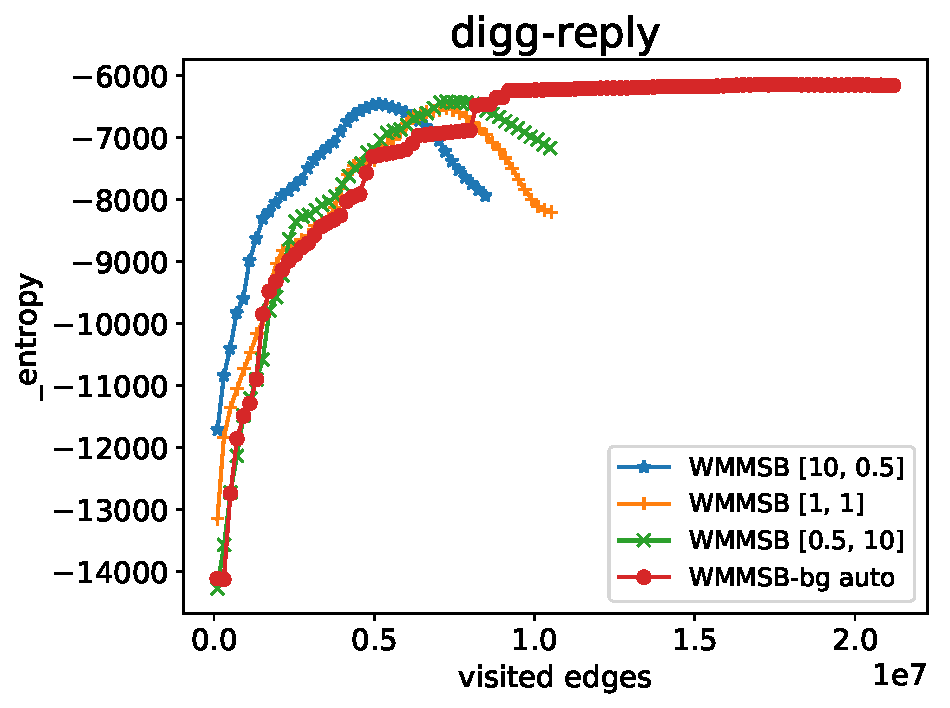
\includegraphics[width=0.32\textwidth]{fig/digg-reply_fig__entropy}               
\end{subfigure}                                                                          
\begin{subfigure}                                                                        
         \centering                                                                      
      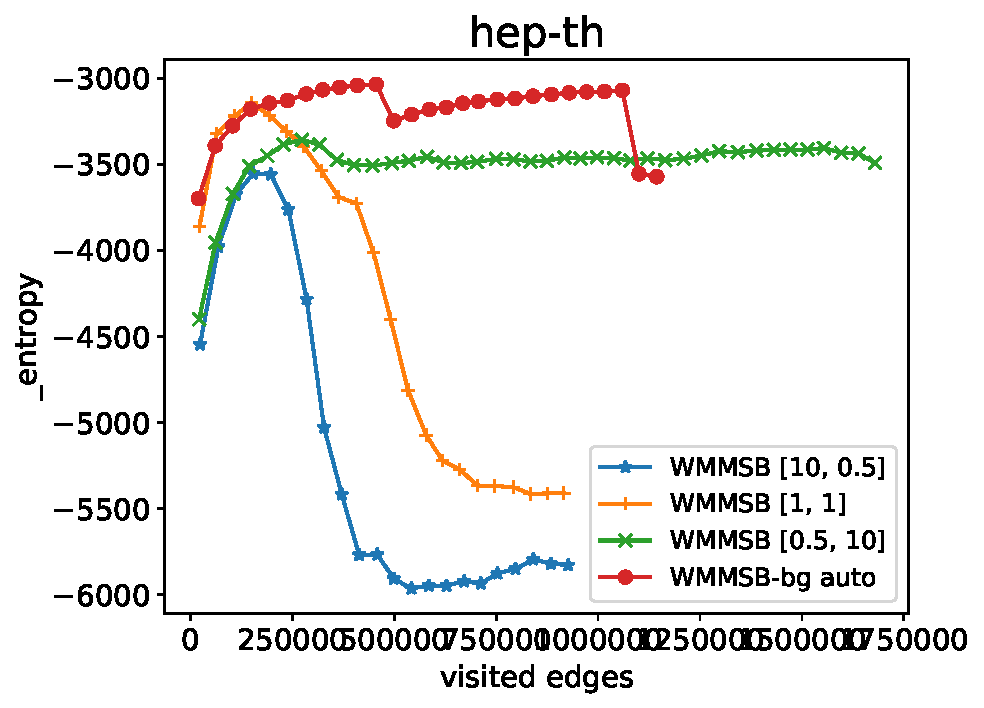
\includegraphics[width=0.32\textwidth]{fig/hep-th_fig__entropy}
\end{subfigure}                                                                          
\begin{subfigure}                                                                        
     \centering                                                                          
         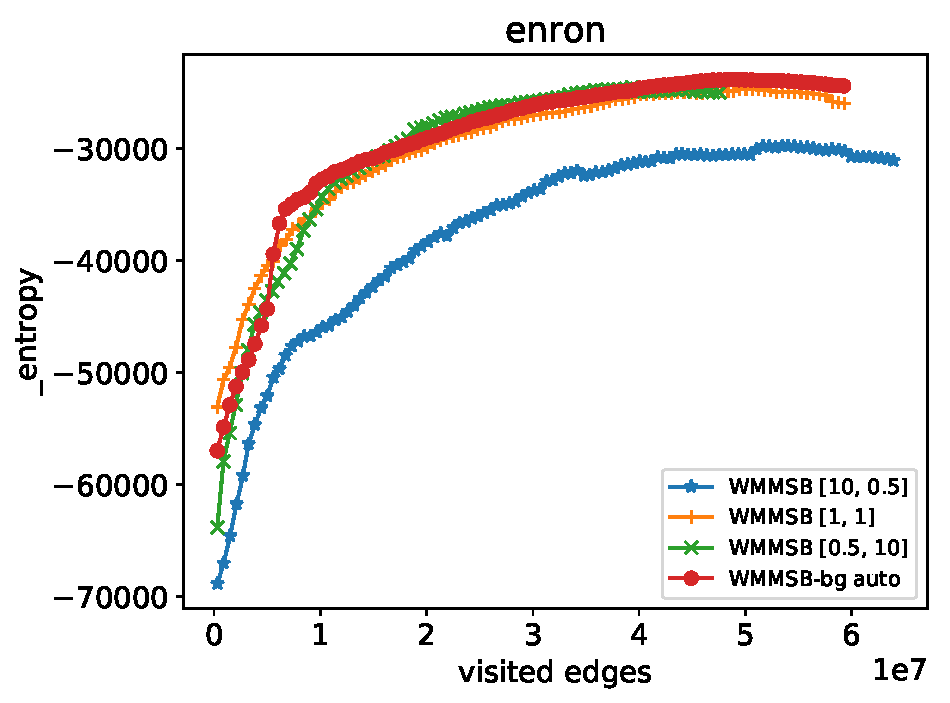
\includegraphics[width=0.32\textwidth]{fig/enron_fig__entropy}
\end{subfigure}
\begin{subfigure}
         \centering
      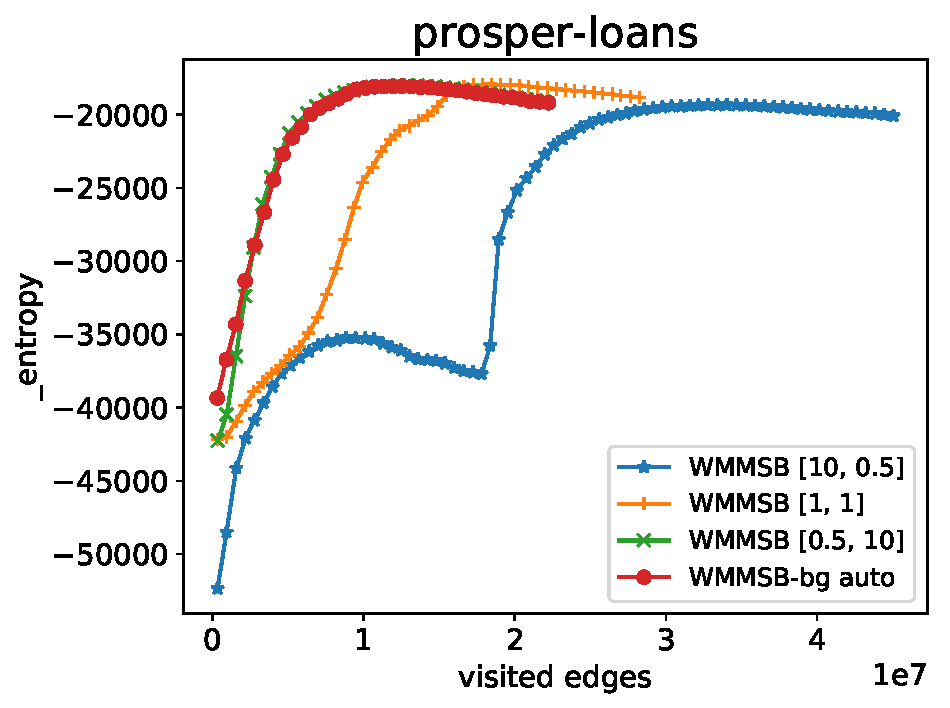
\includegraphics[width=0.32\textwidth]{fig/prosper-loans_fig__entropy}
\end{subfigure}                                                             
\begin{subfigure}                                                           
         \centering                                                         
      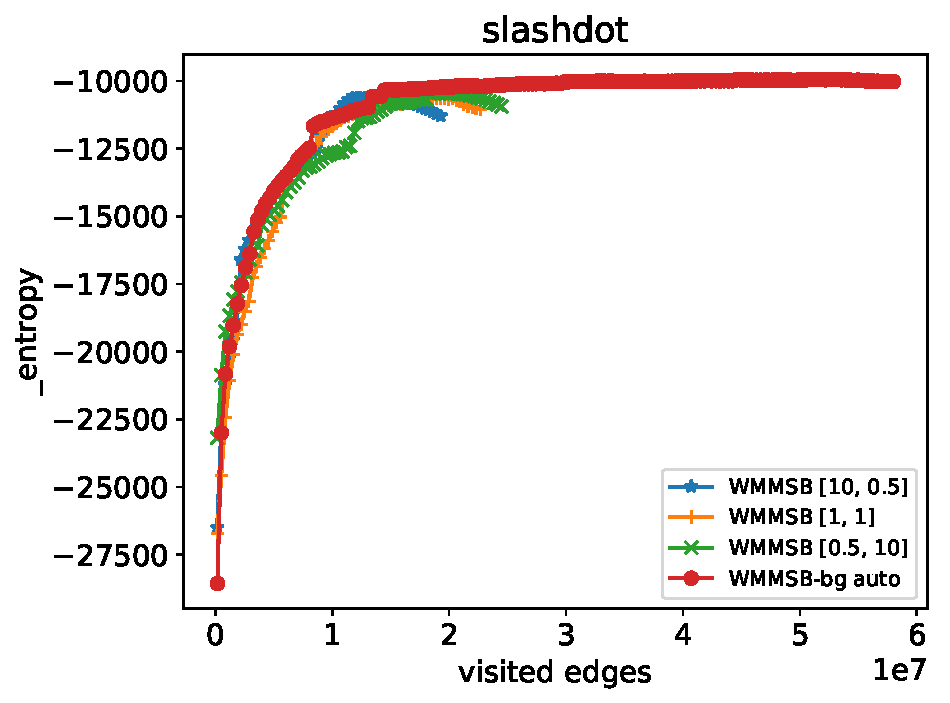
\includegraphics[width=0.32\textwidth]{fig/slashdot_fig__entropy}
\end{subfigure}                                                             
\caption{Log-likehood convergence for WMMSB and WMMSB-bg models. Three different set of hyper-parmeter are used for WMMSB.}


    \label{fig:conv_entropy}
\end{figure}

%Lastly, the complexity of the MMSB-based models with the inference scheme used here is linear in the number of nodes, meaning that it can be sublinear in the number of edges when the network is not too sparse. This has to be contrasted to the complexity of SBM-based models, that is linear in the number of edges. As our implementation, available online\footnote{https://github.com/***/*** (nonymized)}, is in Python whereas the one for SBM models is in C, a direct comparison of the running time of each model is not possible.

%While our implementation is in python, the time convergence of the algorithm is fast and it is even comparable with SBM which is implemented in C. Furthermore, in practice, the algorithm exhibits a sublinear time complexity with the numbers of edges, as shown Table \ref{table:time}.
%
%\begin{table}[h]
%\begin{tabular}{llllll}
%\hline
%                    & MMSB                  & WMMSB-bg              & SBM                  \\
%\hline
%astro-ph      & 361.165 $\pm$ 159.107    & 868.802 $\pm$ 870.965    & 44.646 $\pm$ 4.778      \\
%hep-th        & 170.281 $\pm$ 17.246     & 226.887 $\pm$ 77.84      & 20.366 $\pm$ 4.127      \\
%moreno\_names  & 44.821 $\pm$ 7.717       & 30.362 $\pm$ 11.811      & 5.358 $\pm$ 1.67        \\
%fb\_uc         & 50.927 $\pm$ 17.694      & 66.921 $\pm$ 10.439      & 4.093 $\pm$ 0.907       \\
%digg-reply    & 1803.779 $\pm$ 1100.227  & 2044.334 $\pm$ 1016.157  & 228.661 $\pm$ 81.611    \\
%slashdot      & 4272.667 $\pm$ 1971.346  & 2867.998 $\pm$ 653.092   & 365.437 $\pm$ 82.475    \\
%enron         & 4660.744 $\pm$ 2978.898  & 3544.711 $\pm$ 385.445   & 1313.841 $\pm$ 109.074  \\
%wiki-link     & 13683.093 $\pm$ 6890.663 & 5592.084 $\pm$ 228.13    & 613.841 $\pm$ 113.047   \\
%prosper-loans & 6595.175 $\pm$ 4612.049  & 12255.827 $\pm$ 4878.113 & 1182.409 $\pm$ 183.342  \\
%\hline
%\end{tabular}
%\label{table:time}
%\caption{Inference time in seconds.}
%\end{table}



%
% WSim
%
%For the weighted models, we further measure the capacity to predict right edge counts with a $l_1$ distance between the real count of the test set and the expected count of the models 
%
%\begin{equation*}
%D_{l_1}(D_{test} ||  \{\Thetah, \Phih\}) = \sum_{i,j \in \D_{test}} | y_{ij} - \E[y_{ij}|\Thetah, \Phih] |
%\end{equation*}






